\documentclass[]{article}
\usepackage{lmodern}
\usepackage{amssymb,amsmath}
\usepackage{ifxetex,ifluatex}
\usepackage{fixltx2e} % provides \textsubscript
\ifnum 0\ifxetex 1\fi\ifluatex 1\fi=0 % if pdftex
  \usepackage[T1]{fontenc}
  \usepackage[utf8]{inputenc}
\else % if luatex or xelatex
  \ifxetex
    \usepackage{mathspec}
  \else
    \usepackage{fontspec}
  \fi
  \defaultfontfeatures{Ligatures=TeX,Scale=MatchLowercase}
\fi
% use upquote if available, for straight quotes in verbatim environments
\IfFileExists{upquote.sty}{\usepackage{upquote}}{}
% use microtype if available
\IfFileExists{microtype.sty}{%
\usepackage{microtype}
\UseMicrotypeSet[protrusion]{basicmath} % disable protrusion for tt fonts
}{}
\usepackage[margin=1in]{geometry}
\usepackage{hyperref}
\hypersetup{unicode=true,
            pdftitle={Supplementary for GCalignR: An R package for aligning Gas-Chromatography data},
            pdfauthor={Meinolf Ottensmann, Martin A. Stoffel, Barbara Caspers, Joseph I. Hoffman},
            pdfborder={0 0 0},
            breaklinks=true}
\urlstyle{same}  % don't use monospace font for urls
\usepackage{color}
\usepackage{fancyvrb}
\newcommand{\VerbBar}{|}
\newcommand{\VERB}{\Verb[commandchars=\\\{\}]}
\DefineVerbatimEnvironment{Highlighting}{Verbatim}{commandchars=\\\{\}}
% Add ',fontsize=\small' for more characters per line
\newenvironment{Shaded}{}{}
\newcommand{\KeywordTok}[1]{\textbf{{#1}}}
\newcommand{\DataTypeTok}[1]{\textcolor[rgb]{0.50,0.00,0.00}{{#1}}}
\newcommand{\DecValTok}[1]{\textcolor[rgb]{0.00,0.00,1.00}{{#1}}}
\newcommand{\BaseNTok}[1]{\textcolor[rgb]{0.00,0.00,1.00}{{#1}}}
\newcommand{\FloatTok}[1]{\textcolor[rgb]{0.50,0.00,0.50}{{#1}}}
\newcommand{\ConstantTok}[1]{\textcolor[rgb]{0.00,0.00,0.00}{{#1}}}
\newcommand{\CharTok}[1]{\textcolor[rgb]{1.00,0.00,1.00}{{#1}}}
\newcommand{\SpecialCharTok}[1]{\textcolor[rgb]{1.00,0.00,1.00}{{#1}}}
\newcommand{\StringTok}[1]{\textcolor[rgb]{0.87,0.00,0.00}{{#1}}}
\newcommand{\VerbatimStringTok}[1]{\textcolor[rgb]{0.87,0.00,0.00}{{#1}}}
\newcommand{\SpecialStringTok}[1]{\textcolor[rgb]{0.87,0.00,0.00}{{#1}}}
\newcommand{\ImportTok}[1]{{#1}}
\newcommand{\CommentTok}[1]{\textcolor[rgb]{0.50,0.50,0.50}{\textit{{#1}}}}
\newcommand{\DocumentationTok}[1]{\textcolor[rgb]{0.50,0.50,0.50}{\textit{{#1}}}}
\newcommand{\AnnotationTok}[1]{\textcolor[rgb]{0.50,0.50,0.50}{\textbf{\textit{{#1}}}}}
\newcommand{\CommentVarTok}[1]{\textcolor[rgb]{0.50,0.50,0.50}{\textbf{\textit{{#1}}}}}
\newcommand{\OtherTok}[1]{{#1}}
\newcommand{\FunctionTok}[1]{\textcolor[rgb]{0.00,0.00,0.50}{{#1}}}
\newcommand{\VariableTok}[1]{{#1}}
\newcommand{\ControlFlowTok}[1]{{#1}}
\newcommand{\OperatorTok}[1]{{#1}}
\newcommand{\BuiltInTok}[1]{{#1}}
\newcommand{\ExtensionTok}[1]{{#1}}
\newcommand{\PreprocessorTok}[1]{\textbf{{#1}}}
\newcommand{\AttributeTok}[1]{{#1}}
\newcommand{\RegionMarkerTok}[1]{{#1}}
\newcommand{\InformationTok}[1]{\textcolor[rgb]{0.50,0.50,0.50}{\textbf{\textit{{#1}}}}}
\newcommand{\WarningTok}[1]{\textcolor[rgb]{1.00,0.00,0.00}{\textbf{{#1}}}}
\newcommand{\AlertTok}[1]{\textcolor[rgb]{0.00,1.00,0.00}{\textbf{{#1}}}}
\newcommand{\ErrorTok}[1]{\textcolor[rgb]{1.00,0.00,0.00}{\textbf{{#1}}}}
\newcommand{\NormalTok}[1]{{#1}}
\usepackage{longtable,booktabs}
\usepackage{graphicx,grffile}
\makeatletter
\def\maxwidth{\ifdim\Gin@nat@width>\linewidth\linewidth\else\Gin@nat@width\fi}
\def\maxheight{\ifdim\Gin@nat@height>\textheight\textheight\else\Gin@nat@height\fi}
\makeatother
% Scale images if necessary, so that they will not overflow the page
% margins by default, and it is still possible to overwrite the defaults
% using explicit options in \includegraphics[width, height, ...]{}
\setkeys{Gin}{width=\maxwidth,height=\maxheight,keepaspectratio}
\IfFileExists{parskip.sty}{%
\usepackage{parskip}
}{% else
\setlength{\parindent}{0pt}
\setlength{\parskip}{6pt plus 2pt minus 1pt}
}
\setlength{\emergencystretch}{3em}  % prevent overfull lines
\providecommand{\tightlist}{%
  \setlength{\itemsep}{0pt}\setlength{\parskip}{0pt}}
\setcounter{secnumdepth}{0}
% Redefines (sub)paragraphs to behave more like sections
\ifx\paragraph\undefined\else
\let\oldparagraph\paragraph
\renewcommand{\paragraph}[1]{\oldparagraph{#1}\mbox{}}
\fi
\ifx\subparagraph\undefined\else
\let\oldsubparagraph\subparagraph
\renewcommand{\subparagraph}[1]{\oldsubparagraph{#1}\mbox{}}
\fi

%%% Use protect on footnotes to avoid problems with footnotes in titles
\let\rmarkdownfootnote\footnote%
\def\footnote{\protect\rmarkdownfootnote}

%%% Change title format to be more compact
\usepackage{titling}

% Create subtitle command for use in maketitle
\newcommand{\subtitle}[1]{
  \posttitle{
    \begin{center}\large#1\end{center}
    }
}

\setlength{\droptitle}{-2em}
  \title{Supplementary for ``GCalignR: An R package for aligning
Gas-Chromatography data''}
  \pretitle{\vspace{\droptitle}\centering\huge}
  \posttitle{\par}
  \author{Meinolf Ottensmann, Martin A. Stoffel, Barbara Caspers, Joseph I.
Hoffman}
  \preauthor{\centering\large\emph}
  \postauthor{\par}
  \predate{\centering\large\emph}
  \postdate{\par}
  \date{2016-12-12}


\begin{document}
\maketitle

\begin{verbatim}
## Loading required package: permute
\end{verbatim}

\begin{verbatim}
## Loading required package: lattice
\end{verbatim}

\begin{verbatim}
## This is vegan 2.4-1
\end{verbatim}

\section{Testing GCalignR on empirical
data}\label{testing-gcalignr-on-empirical-data}

\subsection{Data}\label{data}

We demonstrate the usage of \texttt{GcalignR} with two empirical data
sets. A more detailed workthrough tutorial is given in the
\href{../doc/GCalignR_step_by_step.html}{vignette}.

\subsubsection{Bumble bee cephalic
secretions}\label{bumble-bee-cephalic-secretions}

Dellicour and Lecocq (2013) present data for three North America bumble
bee species \emph{Bombus bimaculatus}, \emph{B. ephippiatus} and
\emph{B. flavifrons}. Samples represent cephalic labial gland secretions
and are supposed to show species specific patterns ({\textbf{???}}).
Hence, this in an ideal data set to test both (i) the alignment
efficiency of \textbf{GCalignR} and (ii) the functionality to explore
similarity patterns by multidimensional scaling within one pipeline in
\textbf{R}.

\begin{Shaded}
\begin{Highlighting}[]
\CommentTok{# The data is comprised of 55 samples, distributed as follows:}
\NormalTok{bee_factors <-}\StringTok{ }\KeywordTok{read.csv}\NormalTok{(}\StringTok{"data/d1/Table_S1_factors.csv"}\NormalTok{,}\DataTypeTok{sep =} \StringTok{";"}\NormalTok{)}
\KeywordTok{row.names}\NormalTok{(bee_factors) <-}\StringTok{ }\NormalTok{bee_factors[[}\StringTok{"ID"}\NormalTok{]]}
\KeywordTok{pandoc.table}\NormalTok{(}\KeywordTok{summary}\NormalTok{(bee_factors$Species))}
\end{Highlighting}
\end{Shaded}

\begin{longtable}[]{@{}ccc@{}}
\toprule
\begin{minipage}[b]{0.18\columnwidth}\centering\strut
bimaculatus\strut
\end{minipage} & \begin{minipage}[b]{0.18\columnwidth}\centering\strut
ephippiatus\strut
\end{minipage} & \begin{minipage}[b]{0.18\columnwidth}\centering\strut
flavifrons\strut
\end{minipage}\tabularnewline
\midrule
\endhead
\begin{minipage}[t]{0.18\columnwidth}\centering\strut
24\strut
\end{minipage} & \begin{minipage}[t]{0.18\columnwidth}\centering\strut
20\strut
\end{minipage} & \begin{minipage}[t]{0.18\columnwidth}\centering\strut
11\strut
\end{minipage}\tabularnewline
\bottomrule
\end{longtable}

The chromatogram data was extracted from Table S1 of (Dellicour and
Lecocq 2013) and can be downloaded here:
\{\url{http://onlinelibrary.wiley.com/store/10.1002/jssc.201300388/asset/supinfo/jssc3437-sup-0001-TableS1.zip?v=1\&s=57d5d58273d1d4207e70c72cecd5bba4b1fe95a1}\}\{Supporting
information\}. Prior to excecuting any alignment, the conformity of the
data with the requirements of \texttt{GCalignR}is tested ``behind the
scenes''. Nonetheless, this can be invoked manually by calling the
function \texttt{check\_input}.

\begin{Shaded}
\begin{Highlighting}[]
\KeywordTok{check_input}\NormalTok{(}\DataTypeTok{data =} \StringTok{"data/d1/Table_S1_raw.txt"}\NormalTok{)}
\CommentTok{#> Warning: BEPH06 violate(s) the requirements.}
\CommentTok{#> Warning: Every sample needs to have the same number of values for each}
\CommentTok{#> variable!}
\CommentTok{#> Not all checks have been passed. Read warning messages and change data accordingly}
\end{Highlighting}
\end{Shaded}

The output reveals that sample \emph{BEPH06} is malformed. The last row
contains both area and relative area but no retention time. It is
unclear what this represents. The respective row is removed from the
file we are going to use afterwards.

\begin{Shaded}
\begin{Highlighting}[]
\CommentTok{# By including "list_peaks = T" we can plot the peak distribution }
\CommentTok{# prior to alignment.}
\KeywordTok{check_input}\NormalTok{(}\DataTypeTok{data =} \StringTok{"data/d1/Table_S1_cleaned.txt"}\NormalTok{, }\DataTypeTok{list_peaks =} \NormalTok{T,}
            \DataTypeTok{ylab =} \StringTok{"Peaks"}\NormalTok{, }\DataTypeTok{cex.names =} \FloatTok{0.7}\NormalTok{, }\DataTypeTok{col =} \StringTok{"#E41A1C"}\NormalTok{,}
            \DataTypeTok{main =} \StringTok{"Bumble bees}\CharTok{\textbackslash{}n}\StringTok{ n = 55"}\NormalTok{)}
\CommentTok{#> All checks passed!}
\CommentTok{#> Ready for processing with align_chromatograms}
\end{Highlighting}
\end{Shaded}

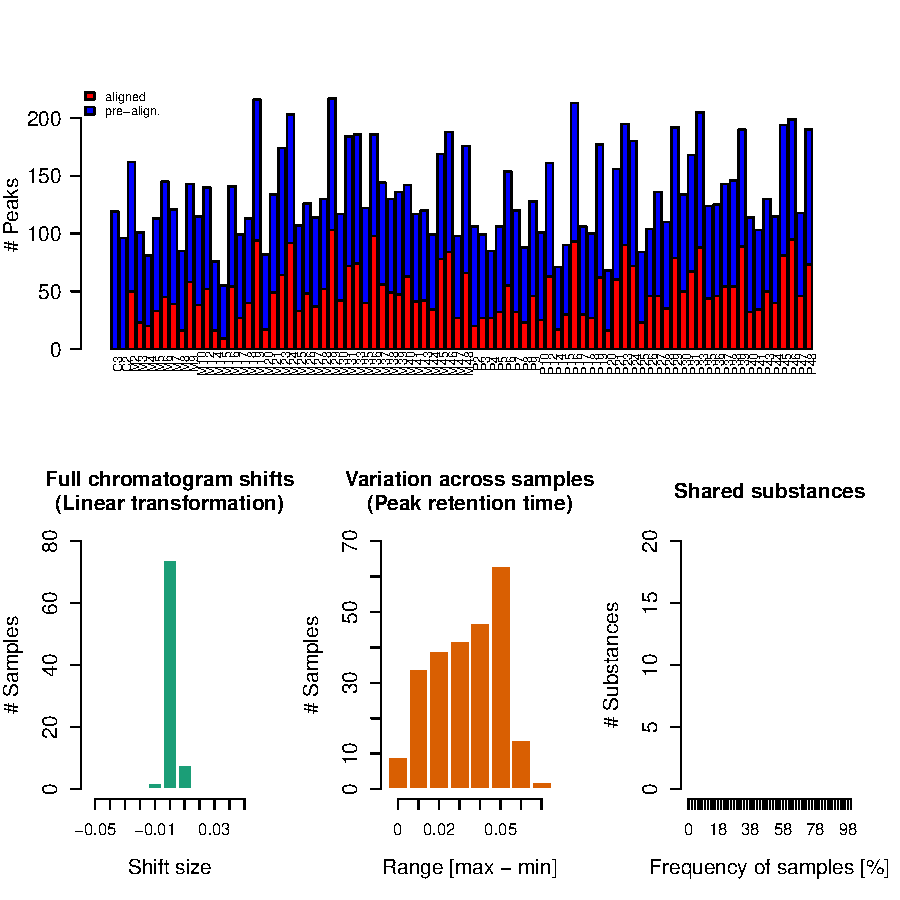
\includegraphics{Supplementary_1_files/figure-latex/unnamed-chunk-5-1.pdf}

\subsubsection{\texorpdfstring{Antarctic fur seal \emph{Arctocephalus
gazella} skin
swabs}{Antarctic fur seal Arctocephalus gazella skin swabs}}\label{antarctic-fur-seal-arctocephalus-gazella-skin-swabs}

The second data set is comprised of skin swabs of 41 mother-pup pairs of
Antarctic fur seals \emph{Arctocephalus gazella} which among other
things were shown to encode the membership to a breeding colony (Stoffel
et al. 2015).

\begin{Shaded}
\begin{Highlighting}[]
\KeywordTok{check_input}\NormalTok{(}\DataTypeTok{data =} \NormalTok{peak_data, }\DataTypeTok{list_peaks =} \NormalTok{T, }\DataTypeTok{cex.names =} \FloatTok{0.6}\NormalTok{,}
            \DataTypeTok{ylab =} \StringTok{"Peaks"}\NormalTok{, }\DataTypeTok{col =} \StringTok{"#377EB8"}\NormalTok{, }\DataTypeTok{main =} \StringTok{"Antarctic fur seal}\CharTok{\textbackslash{}n}\StringTok{ n = 82"}\NormalTok{)}
\CommentTok{#> All checks passed!}
\CommentTok{#> Ready for processing with align_chromatograms}
\end{Highlighting}
\end{Shaded}

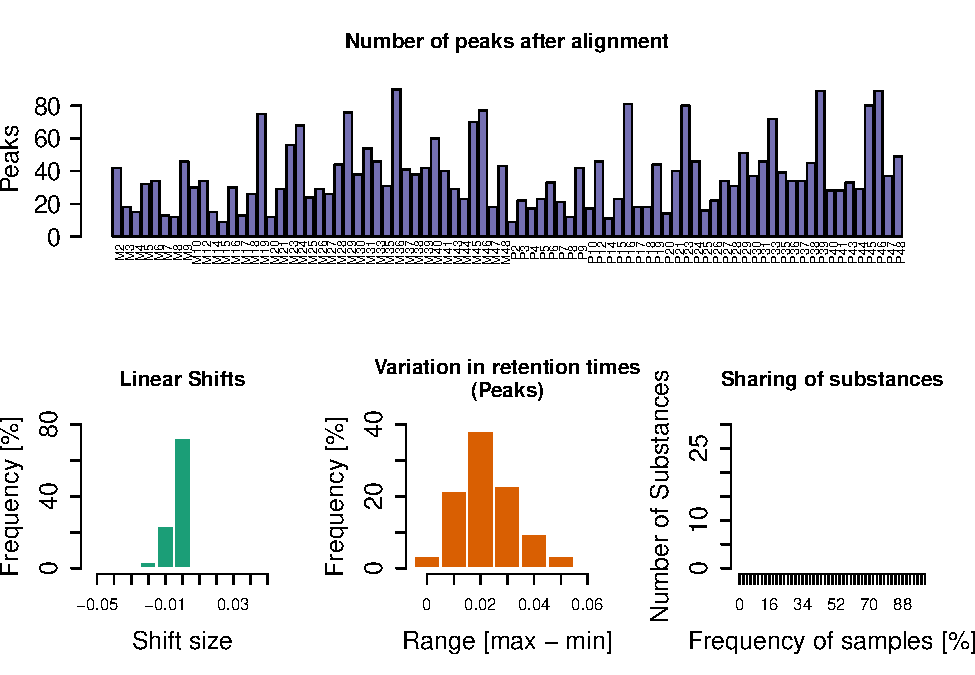
\includegraphics{Supplementary_1_files/figure-latex/unnamed-chunk-6-1.pdf}

\subsection{Alignment}\label{alignment}

\begin{itemize}
\tightlist
\item
  Aligning the bumblee bee data
\end{itemize}

\begin{Shaded}
\begin{Highlighting}[]
\NormalTok{bee_aligned <-}\StringTok{ }\KeywordTok{align_chromatograms}\NormalTok{(}\DataTypeTok{data =} \StringTok{"data/d1/Table_S1_cleaned.txt"}\NormalTok{,}
                    \DataTypeTok{conc_col_name =} \StringTok{"Area"}\NormalTok{,}
                    \DataTypeTok{max_diff_peak2mean =} \FloatTok{0.02}\NormalTok{,}
                    \DataTypeTok{min_diff_peak2peak =} \FloatTok{0.05}\NormalTok{,}
                    \DataTypeTok{rt_col_name =} \StringTok{"RT"}\NormalTok{,}
                    \DataTypeTok{delete_single_peak =} \NormalTok{T,}
                    \DataTypeTok{iterations =} \DecValTok{1}\NormalTok{)}
\KeywordTok{save}\NormalTok{(bee_aligned, }\DataTypeTok{file =} \StringTok{"data/d1/bee_aligned.RData"}\NormalTok{)}
\end{Highlighting}
\end{Shaded}

\begin{Shaded}
\begin{Highlighting}[]
\CommentTok{# aligned data}
\KeywordTok{load}\NormalTok{(}\DataTypeTok{file =} \StringTok{"data/d1/bee_aligned.RData"}\NormalTok{)}
\end{Highlighting}
\end{Shaded}

\begin{itemize}
\tightlist
\item
  Exploring species similarites with non-metric multidimensional scaling
  (NMDS)
\end{itemize}

\begin{Shaded}
\begin{Highlighting}[]
\CommentTok{# normalise abundancies within samples}
\NormalTok{bee_scent <-}\StringTok{ }\NormalTok{GCalignR::}\KeywordTok{norm_peaks}\NormalTok{(bee_aligned,}\DataTypeTok{conc_col_name =} \StringTok{"Area"}\NormalTok{,}\DataTypeTok{rt_col_name =} \StringTok{"RT"}\NormalTok{,}\DataTypeTok{out =} \StringTok{"data.frame"}\NormalTok{)}
\CommentTok{# Log + 1 Transformation}
\NormalTok{bee_scent <-}\StringTok{ }\KeywordTok{log}\NormalTok{(bee_scent +}\StringTok{ }\DecValTok{1}\NormalTok{) }
\NormalTok{bee_scent <-}\StringTok{ }\NormalTok{bee_scent[}\KeywordTok{match}\NormalTok{(}\KeywordTok{row.names}\NormalTok{(bee_factors),}\KeywordTok{row.names}\NormalTok{(bee_scent)),] }
\CommentTok{# NMDS using bray-curtis in vegan}
\NormalTok{bee_scent_nmds <-}\StringTok{ }\NormalTok{vegan::}\KeywordTok{metaMDS}\NormalTok{(}\DataTypeTok{comm =} \NormalTok{bee_scent,}\DataTypeTok{trymax =} \DecValTok{9999}\NormalTok{) }
\CommentTok{# Get the coordinates}
\NormalTok{bee_scent_nmds <-}\StringTok{ }\KeywordTok{as.data.frame}\NormalTok{(bee_scent_nmds$points) }
\NormalTok{bee_scent_nmds <-}\StringTok{ }\KeywordTok{cbind}\NormalTok{(bee_scent_nmds,}\DataTypeTok{Species =} \NormalTok{bee_factors[[}\StringTok{"Species"}\NormalTok{]])  }
\end{Highlighting}
\end{Shaded}

\begin{itemize}
\tightlist
\item
  Visualisation using \texttt{ggplot2}
\end{itemize}

\begin{Shaded}
\begin{Highlighting}[]
\NormalTok{ggplot2::}\KeywordTok{ggplot}\NormalTok{(}\DataTypeTok{data =} \NormalTok{bee_scent_nmds,ggplot2::}\KeywordTok{aes}\NormalTok{(MDS1,MDS2,}\DataTypeTok{color =} \NormalTok{Species)) +}
\NormalTok{ggplot2::}\KeywordTok{geom_point}\NormalTok{(}\DataTypeTok{size =} \DecValTok{3}\NormalTok{) +}\StringTok{ }
\NormalTok{ggplot2::}\KeywordTok{stat_ellipse}\NormalTok{(}\DataTypeTok{size =} \DecValTok{2}\NormalTok{) +}\StringTok{ }
\NormalTok{ggplot2::}\KeywordTok{labs}\NormalTok{(}\DataTypeTok{title =} \StringTok{""}\NormalTok{, }\DataTypeTok{x =} \StringTok{"MDS1"}\NormalTok{, }\DataTypeTok{y =} \StringTok{"MDS2"}\NormalTok{) +}
\NormalTok{ggplot2::}\KeywordTok{theme_bw}\NormalTok{(}\DataTypeTok{base_size =} \DecValTok{14}\NormalTok{) +}\StringTok{ }
\NormalTok{ggplot2::}\KeywordTok{theme}\NormalTok{(}\DataTypeTok{axis.ticks =} \KeywordTok{element_blank}\NormalTok{(), }\DataTypeTok{axis.text =} \KeywordTok{element_blank}\NormalTok{()) +}
\StringTok{    }\KeywordTok{scale_colour_manual}\NormalTok{(}\DataTypeTok{values =} \NormalTok{RColorBrewer::}\KeywordTok{brewer.pal}\NormalTok{(}\DecValTok{3}\NormalTok{,}\StringTok{"Dark2"}\NormalTok{), }
    \DataTypeTok{name =} \StringTok{""}\NormalTok{,}
    \DataTypeTok{breaks =} \KeywordTok{c}\NormalTok{(}\StringTok{"bimaculatus"}\NormalTok{, }\StringTok{"ephippiatus"}\NormalTok{, }\StringTok{"flavifrons"}\NormalTok{),}
    \DataTypeTok{labels =} \KeywordTok{c}\NormalTok{(}\StringTok{"Bombus bimaculatus"}\NormalTok{,}\StringTok{"B. ephippiatus"}\NormalTok{,}\StringTok{"B. flavifrons"}\NormalTok{),}
    \DataTypeTok{guide =} \KeywordTok{guide_legend}\NormalTok{(}\DataTypeTok{label.theme =} \KeywordTok{element_text}\NormalTok{(}
    \DataTypeTok{face =} \StringTok{"italic"}\NormalTok{, }\DataTypeTok{angle =} \DecValTok{0}\NormalTok{, }\DataTypeTok{size =} \DecValTok{11}\NormalTok{)))}
\end{Highlighting}
\end{Shaded}

\includegraphics{Supplementary_1_files/figure-latex/unnamed-chunk-10-1.pdf}
* Multivariate statistics using \texttt{adonis} reveal a highly
significant clustering by species

\begin{Shaded}
\begin{Highlighting}[]
\NormalTok{vegan::}\KeywordTok{adonis}\NormalTok{(bee_scent ~}\StringTok{ }\NormalTok{bee_factors$Species,}\DataTypeTok{permutations =} \DecValTok{999}\NormalTok{)}
\CommentTok{#> }
\CommentTok{#> Call:}
\CommentTok{#> vegan::adonis(formula = bee_scent ~ bee_factors$Species, permutations = 999) }
\CommentTok{#> }
\CommentTok{#> Permutation: free}
\CommentTok{#> Number of permutations: 999}
\CommentTok{#> }
\CommentTok{#> Terms added sequentially (first to last)}
\CommentTok{#> }
\CommentTok{#>                     Df SumsOfSqs MeanSqs F.Model      R2 Pr(>F)    }
\CommentTok{#> bee_factors$Species  2    7.0089  3.5045   32.73 0.55729  0.001 ***}
\CommentTok{#> Residuals           52    5.5678  0.1071         0.44271           }
\CommentTok{#> Total               54   12.5768                 1.00000           }
\CommentTok{#> ---}
\CommentTok{#> Signif. codes:  0 '***' 0.001 '**' 0.01 '*' 0.05 '.' 0.1 ' ' 1}
\end{Highlighting}
\end{Shaded}

\begin{center}\rule{0.5\linewidth}{\linethickness}\end{center}

R version and platform.

\begin{Shaded}
\begin{Highlighting}[]
\KeywordTok{sessionInfo}\NormalTok{()}
\CommentTok{#> R version 3.3.2 (2016-10-31)}
\CommentTok{#> Platform: x86_64-w64-mingw32/x64 (64-bit)}
\CommentTok{#> Running under: Windows 10 x64 (build 14393)}
\CommentTok{#> }
\CommentTok{#> locale:}
\CommentTok{#> [1] LC_COLLATE=German_Germany.1252  LC_CTYPE=German_Germany.1252   }
\CommentTok{#> [3] LC_MONETARY=German_Germany.1252 LC_NUMERIC=C                   }
\CommentTok{#> [5] LC_TIME=German_Germany.1252    }
\CommentTok{#> }
\CommentTok{#> attached base packages:}
\CommentTok{#> [1] stats     graphics  grDevices utils     datasets  methods   base     }
\CommentTok{#> }
\CommentTok{#> other attached packages:}
\CommentTok{#> [1] vegan_2.4-1         lattice_0.20-33     permute_0.9-0      }
\CommentTok{#> [4] ggplot2_2.1.0       pander_0.6.0        bibtex_0.4.0       }
\CommentTok{#> [7] knitcitations_1.0-2 GCalignR_0.0.9000  }
\CommentTok{#> }
\CommentTok{#> loaded via a namespace (and not attached):}
\CommentTok{#>  [1] Rcpp_0.12.4        formatR_1.4        RColorBrewer_1.1-2}
\CommentTok{#>  [4] plyr_1.8.3         bitops_1.0-6       tools_3.3.2       }
\CommentTok{#>  [7] digest_0.6.10      lubridate_1.6.0    evaluate_0.9      }
\CommentTok{#> [10] tibble_1.1         gtable_0.2.0       nlme_3.1-127      }
\CommentTok{#> [13] mgcv_1.8-12        Matrix_1.2-6       yaml_2.1.13       }
\CommentTok{#> [16] parallel_3.3.2     RefManageR_0.13.1  stringr_1.1.0     }
\CommentTok{#> [19] httr_1.2.1         knitr_1.14         cluster_2.0.4     }
\CommentTok{#> [22] grid_3.3.2         R6_2.1.2           XML_3.98-1.5      }
\CommentTok{#> [25] rmarkdown_1.1      RJSONIO_1.3-0      reshape2_1.4.2    }
\CommentTok{#> [28] readr_1.0.0        magrittr_1.5       scales_0.4.0      }
\CommentTok{#> [31] htmltools_0.3.5    MASS_7.3-45        assertthat_0.1    }
\CommentTok{#> [34] colorspace_1.2-6   labeling_0.3       stringi_1.1.1     }
\CommentTok{#> [37] RCurl_1.95-4.8     munsell_0.4.3}
\end{Highlighting}
\end{Shaded}

\begin{center}\rule{0.5\linewidth}{\linethickness}\end{center}

\subsection*{References}\label{references}
\addcontentsline{toc}{subsection}{References}

\hypertarget{refs}{}
\hypertarget{ref-Dellicour.2013}{}
Dellicour, Simon, and Thomas Lecocq. 2013. ``GCALIGNER 1.0: An Alignment
Program to Compute a Multiple Sample Comparison Data Matrix from Large
Eco-Chemical Datasets Obtained by Gc.'' \emph{Journal of Separation
Science} 36 (19): 3206--9.
doi:\href{https://doi.org/10.1002/jssc.201300388}{10.1002/jssc.201300388}.

\hypertarget{ref-Stoffel.2015}{}
Stoffel, Martin A., Barbara A. Caspers, Jaume Forcada, Athina
Giannakara, Markus Baier, Luke Eberhart-Phillips, Caroline Müller, and
Joseph I. Hoffman. 2015. ``Chemical Fingerprints Encode
Mother--offspring Similarity, Colony Membership, Relatedness, and
Genetic Quality in Fur Seals.'' \emph{Proceedings of the National
Academy of Sciences} 112 (36): E5005--E5012.


\end{document}
